%  LaTeX support: latex@mdpi.com 
%  For support, please attach all files needed for compiling as well as the log file, and specify your operating system, LaTeX version, and LaTeX editor.
\PassOptionsToPackage{dvipsnames}{xcolor}
%=================================================================
\documentclass[journal,article,submit,pdftex,moreauthors]{Definitions/mdpi}
%\renewcommand{\linenumbers}{}
\usepackage{comment}
\usepackage{pgfplots}
\pgfplotsset{compat=1.18}
\usepackage{pgf-pie}  
\usepackage[dvipsnames]{xcolor}
\usepackage{marginnote}
\usepackage{graphicx}
\usepackage{subcaption}
% For posting an early version of this manuscript as a preprint, you may use "preprints" as the journal and change "submit" to "accept". The document class line would be, e.g., \documentclass[preprints,article,accept,moreauthors,pdftex]{mdpi}. This is especially recommended for submission to arXiv, where line numbers should be removed before posting. For preprints.org, the editorial staff will make this change immediately prior to posting.

%--------------------
% Class Options:
%--------------------
%----------
% journal
%----------
% Choose between the following MDPI journals:
% acoustics, actuators, addictions, admsci, adolescents, aerospace, agriculture, agriengineering, agronomy, ai, algorithms, allergies, alloys, analytica, animals, antibiotics, antibodies, antioxidants, applbiosci, appliedchem, appliedmath, applmech, applmicrobiol, applnano, applsci, aquacj, architecture, arts, asc, asi, astronomy, atmosphere, atoms, audiolres, automation, axioms, bacteria, batteries, bdcc, behavsci, beverages, biochem, bioengineering, biologics, biology, biomass, biomechanics, biomed, biomedicines, biomedinformatics, biomimetics, biomolecules, biophysica, biosensors, biotech, birds, bloods, blsf, brainsci, breath, buildings, businesses, cancers, carbon, cardiogenetics, catalysts, cells, ceramics, challenges, chemengineering, chemistry, chemosensors, chemproc, children, chips, cimb, civileng, cleantechnol, climate, clinpract, clockssleep, cmd, coasts, coatings, colloids, colorants, commodities, compounds, computation, computers, condensedmatter, conservation, constrmater, cosmetics, covid, crops, cryptography, crystals, csmf, ctn, curroncol, currophthalmol, cyber, dairy, data, dentistry, dermato, dermatopathology, designs, diabetology, diagnostics, dietetics, digital, disabilities, diseases, diversity, dna, drones, dynamics, earth, ebj, ecologies, econometrics, economies, education, ejihpe, electricity, electrochem, electronicmat, electronics, encyclopedia, endocrines, energies, eng, engproc, ent, entomology, entropy, environments, environsciproc, epidemiologia, epigenomes, est, fermentation, fibers, fintech, fire, fishes, fluids, foods, forecasting, forensicsci, forests, foundations, fractalfract, fuels, futureinternet, futureparasites, futurepharmacol, futurephys, futuretransp, galaxies, games, gases, gastroent, gastrointestdisord, gels, genealogy, genes, geographies, geohazards, geomatics, geosciences, geotechnics, geriatrics, hazardousmatters, healthcare, hearts, hemato, heritage, highthroughput, histories, horticulturae, humanities, humans, hydrobiology, hydrogen, hydrology, hygiene, idr, ijerph, ijfs, ijgi, ijms, ijns, ijtm, ijtpp, immuno, informatics, information, infrastructures, inorganics, insects, instruments, inventions, iot, j, jal, jcdd, jcm, jcp, jcs, jdb, jeta, jfb, jfmk, jimaging, jintelligence, jlpea, jmmp, jmp, jmse, jne, jnt, jof, joitmc, jor, journalmedia, jox, jpm, jrfm, jsan, jtaer, jzbg, kidney, kidneydial, knowledge, land, languages, laws, life, liquids, literature, livers, logics, logistics, lubricants, lymphatics, machines, macromol, magnetism, magnetochemistry, make, marinedrugs, materials, materproc, mathematics, mca, measurements, medicina, medicines, medsci, membranes, merits, metabolites, metals, meteorology, methane, metrology, micro, microarrays, microbiolres, micromachines, microorganisms, microplastics, minerals, mining, modelling, molbank, molecules, mps, msf, mti, muscles, nanoenergyadv, nanomanufacturing, nanomaterials, ncrna, network, neuroglia, neurolint, neurosci, nitrogen, notspecified, nri, nursrep, nutraceuticals, nutrients, obesities, oceans, ohbm, onco, oncopathology, optics, oral, organics, organoids, osteology, oxygen, parasites, parasitologia, particles, pathogens, pathophysiology, pediatrrep, pharmaceuticals, pharmaceutics, pharmacoepidemiology, pharmacy, philosophies, photochem, photonics, phycology, physchem, physics, physiologia, plants, plasma, pollutants, polymers, polysaccharides, poultry, powders, preprints, proceedings, processes, prosthesis, proteomes, psf, psych, psychiatryint, psychoactives, publications, quantumrep, quaternary, qubs, radiation, reactions, recycling, regeneration, religions, remotesensing, reports, reprodmed, resources, rheumato, risks, robotics, ruminants, safety, sci, scipharm, seeds, sensors, separations, sexes, signals, sinusitis, skins, smartcities, sna, societies, socsci, software, soilsystems, solar, solids, sports, standards, stats, stresses, surfaces, surgeries, suschem, sustainability, symmetry, synbio, systems, taxonomy, technologies, telecom, test, textiles, thalassrep, thermo, tomography, tourismhosp, toxics, toxins, transplantology, transportation, traumacare, traumas, tropicalmed, universe, urbansci, uro, vaccines, vehicles, venereology, vetsci, vibration, viruses, vision, waste, water, wem, wevj, wind, women, world, youth, zoonoticdis 

%---------
% article
%---------
% The default type of manuscript is "article", but can be replaced by: 
% abstract, addendum, article, book, bookreview, briefreport, casereport, comment, commentary, communication, conferenceproceedings, correction, conferencereport, entry, expressionofconcern, extendedabstract, datadescriptor, editorial, essay, erratum, hypothesis, interestingimage, obituary, opinion, projectreport, reply, retraction, review, perspective, protocol, shortnote, studyprotocol, systematicreview, supfile, technicalnote, viewpoint, guidelines, registeredreport, tutorial
% supfile = supplementary materials

%----------
% submit
%----------
% The class option "submit" will be changed to "accept" by the Editorial Office when the paper is accepted. This will only make changes to the frontpage (e.g., the logo of the journal will get visible), the headings, and the copyright information. Also, line numbering will be removed. Journal info and pagination for accepted papers will also be assigned by the Editorial Office.

%------------------
% moreauthors
%------------------
% If there is only one author the class option oneauthor should be used. Otherwise use the class option moreauthors.

%---------
% pdftex
%---------
% The option pdftex is for use with pdfLaTeX. If eps figures are used, remove the option pdftex and use LaTeX and dvi2pdf.

%=================================================================
% MDPI internal commands
\firstpage{1} 
\makeatletter 
\setcounter{page}{\@firstpage} 
\makeatother
\pubvolume{1}
\issuenum{1}
\articlenumber{0}
\pubyear{2022}
\copyrightyear{2022}
%\externaleditor{Academic Editor: Firstname Lastname}
\datereceived{} 
%\daterevised{} % Only for the journal Acoustics
\dateaccepted{} 
\datepublished{} 
%\datecorrected{} % Corrected papers include a "Corrected: XXX" date in the original paper.
%\dateretracted{} % Corrected papers include a "Retracted: XXX" date in the original paper.
\hreflink{https://doi.org/} % If needed use \linebreak
%\doinum{}
%------------------------------------------------------------------
% The following line should be uncommented if the LaTeX file is uploaded to arXiv.org
%\pdfoutput=1

%=================================================================
% Add packages and commands here. The following packages are loaded in our class file: fontenc, inputenc, calc, indentfirst, fancyhdr, graphicx, epstopdf, lastpage, ifthen, lineno, float, amsmath, setspace, enumitem, mathpazo, booktabs, titlesec, etoolbox, tabto, xcolor, soul, multirow, microtype, tikz, totcount, changepage, attrib, upgreek, cleveref, amsthm, hyphenat, natbib, hyperref, footmisc, url, geometry, newfloat, caption

%=================================================================
%% Please use the following mathematics environments: Theorem, Lemma, Corollary, Proposition, Characterization, Property, Problem, Example, ExamplesandDefinitions, Hypothesis, Remark, Definition, Notation, Assumption
%% For proofs, please use the proof environment (the amsthm package is loaded by the MDPI class).

%=================================================================
% Full title of the paper (Capitalized)
\Title{A review on trending Machine Learning techniques for type 2 diabetes.}

% MDPI internal command: Title for citation in the left column
\TitleCitation{Title}

% Author Orchid ID: enter ID or remove command
\newcommand{\orcidauthorA}{0000-0000-0000-000X} % Add \orcidA{} behind the author's name
%\newcommand{\orcidauthorB}{0000-0000-0000-000X} % Add \orcidB{} behind the author's name

% Authors, for the paper (add full first names)
\Author{Firstname Lastname $^{1,\dagger,\ddagger}$\orcidA{}, Firstname Lastname $^{2,\ddagger}$ and Firstname Lastname $^{2,}$*}

%\longauthorlist{yes}

% MDPI internal command: Authors, for metadata in PDF
\AuthorNames{Firstname Lastname, Firstname Lastname and Firstname Lastname}

% MDPI internal command: Authors, for citation in the left column
\AuthorCitation{Lastname, F.; Lastname, F.; Lastname, F.}
% If this is a Chicago style journal: Lastname, Firstname, Firstname Lastname, and Firstname Lastname.

% Affiliations / Addresses (Add [1] after \address if there is only one affiliation.)
\address{%
$^{1}$ \quad Affiliation 1; e-mail@e-mail.com\\
$^{2}$ \quad Affiliation 2; e-mail@e-mail.com}

% Contact information of the corresponding author
\corres{Correspondence: e-mail@e-mail.com; Tel.: (optional; include country code; if there are multiple corresponding authors, add author initials) +xx-xxxx-xxx-xxxx (F.L.)}

% Current address and/or shared authorship
\firstnote{Current address: Affiliation 3.} 
\secondnote{These authors contributed equally to this work.}
% The commands \thirdnote{} till \eighthnote{} are available for further notes

%\simplesumm{} % Simple summary

%\conference{} % An extended version of a conference paper

% Abstract (Do not insert blank lines, i.e. \\) 
\abstract{Diabetes is a chronic disease which is characterized by elevated blood glycose levels, causing damages to human organs and tissues, worsen quality
of life, and even having lethal implications. Last years, medicine have been in pace with data science, in the sense that its digital retransformation 
led to electronic health records (EHRs) collection of indivudials, patients and healthy ones. Thus, plenty of indivudial research articles as well as 
systematic reviews have been conducted in order to produce innovative findings and summarize the current development, respecitively. In this study, a
detailed review is conducted in the context of T2D mellitus and Machine Learning, examining relatively new publications using tabular data,
demonstrating the relevant use cases, the workflows during model building and the candidate predictors. Our findings showed that Gradient Boosting and Tree based models
are the most successfull ones, SHAPley and Wrapper algorithms are quite popular feature interpretation and evaluation methods highlighting urinary results and
dietary as asceding diabetes predictors apart from the classical invasive ones. These results could be offer easier management of the diabetes condition and
open new research areas. 
}


% Keywords
\keyword{Diabetes Mellitus; Machine Learning; Electronic Health Records; Non invasive decision support;} 

% The fields PACS, MSC, and JEL may be left empty or commented out if not applicable
%\PACS{J0101}
%\MSC{}
%\JEL{}

%%%%%%%%%%%%%%%%%%%%%%%%%%%%%%%%%%%%%%%%%%
% Only for the journal Diversity
%\LSID{\url{http://}}

%%%%%%%%%%%%%%%%%%%%%%%%%%%%%%%%%%%%%%%%%%
% Only for the journal Applied Sciences
%\featuredapplication{Authors are encouraged to provide a concise description of the specific application or a potential application of the work. This section is not mandatory.}
%%%%%%%%%%%%%%%%%%%%%%%%%%%%%%%%%%%%%%%%%%

%%%%%%%%%%%%%%%%%%%%%%%%%%%%%%%%%%%%%%%%%%
% Only for the journal Data
%\dataset{DOI number or link to the deposited data set if the data set is published separately. If the data set shall be published as a supplement to this paper, this field will be filled by the journal editors. In this case, please submit the data set as a supplement.}
%\datasetlicense{License under which the data set is made available (CC0, CC-BY, CC-BY-SA, CC-BY-NC, etc.)}

%%%%%%%%%%%%%%%%%%%%%%%%%%%%%%%%%%%%%%%%%%
% Only for the journal Toxins
%\keycontribution{The breakthroughs or highlights of the manuscript. Authors can write one or two sentences to describe the most important part of the paper.}

%%%%%%%%%%%%%%%%%%%%%%%%%%%%%%%%%%%%%%%%%%
% Only for the journal Encyclopedia
%\encyclopediadef{For entry manuscripts only: please provide a brief overview of the entry title instead of an abstract.}

%%%%%%%%%%%%%%%%%%%%%%%%%%%%%%%%%%%%%%%%%%
\begin{document}

%%%%%%%%%%%%%%%%%%%%%%%%%%%%%%%%%%%%%%%%%%
%\setcounter{section}{-1} %% Remove this when starting to work on the template.
%\section{How to Use this Template}

%The template details the sections that can be used in a manuscript. Note that the order and names of article sections may differ from the requirements of the journal (e.g., the positioning of the Materials and Methods section). Please check the instructions on the authors' page of the journal to verify the correct order and names. For any questions, please contact the editorial office of the journal or support@mdpi.com. For LaTeX-related questions please contact latex@mdpi.com.%\endnote{This is an endnote.} % To use endnotes, please un-comment \printendnotes below (before References). Only journal Laws uses \footnote.

% The order of the section titles is: Introduction, Materials and Methods, Results, Discussion, Conclusions for these journals: aerospace,algorithms,antibodies,antioxidants,atmosphere,axioms,biomedicines,carbon,crystals,designs,diagnostics,environments,fermentation,fluids,forests,fractalfract,informatics,information,inventions,jfmk,jrfm,lubricants,neonatalscreening,neuroglia,particles,pharmaceutics,polymers,processes,technologies,viruses,vision
%\section{title}{
%	A single paragraph of about 200 words maximum. For research articles, abstracts should give a pertinent overview of the work. We strongly encourage authors to use the following style of structured abstracts, but without headings: (1) Background: place the question addressed in a broad context and highlight the purpose of the study; (2) Methods: describe briefly the main methods or treatments applied; (3) Results: summarize the article's main findings; (4) Conclusions: indicate the main conclusions or interpretations. The abstract should be an objective representation of the article, it must not contain results which are not presented and substantiated in the main text and should not exaggerate the main conclusions.
%}

\section{Introduction}
Diabetes is an increasing chronic disease that affects people health and quality of life. The IDF Diabetes Atlas (2021) reports
that 10.5\% of the adult population (20-79 years) has diabetes, with almost half unaware that they are living with the condition,
while by 2045 1 in 8 adults, approximately 783 million, will be living with diabetes, an increase of 46\% \cite{idf}. 
Over 90\% of people with diabetes have type 2 diabetes, which is driven by socio-economic, demographic, environmental, and 
genetic factors. On the other hand, Machine Learning has been a powerfull tool for prediction of events, among them medical 
related, as well as for the analysis of massive data and extraction of usefull knowledge. To this end, many studies have been 
conducted for the prediction of diabetes as well as for the identification of factors significantly contributing positive or negative
to its management \cite{KAVAKIOTIS2017104,Fregoso}. These studies address diabetes case in a broad context, ranging from 
Diabetic Complications, Genetic Background and Environment to Drugs and Therapies, and Health Care and Management regarding diabetes,
and reaching deep learning with image analysis regarding Machine Learning, offering not so detailed insights about the methodologies.
In this paper we review a variety of recent research papers towards diabetes diagnosis, diabetes long term prediction and relevant biomarkers
regression, using tabular data coming from questionnairies, biometric, laboratory, physical examinations and dietary habits. 
Our aim is to analyze each paper for its methodology towards data preprocessing, feature selection, model building, evaluation 
and feature importance extraction, with an ultimate goal to unveil patterns, best models and new non invasive predictors, opening
new research areas. 
 
%The introduction should  \cite{LAMA2021e07419}, \cite{KAVAKIOTIS2017104}, \cite{kopitar2020early}, \cite{Howlader}, \cite{ijerph18063317}, \cite{Lai}, \cite{fazakis}, \cite{Zou}, \cite{DeSilva}, \cite{Dinh}, \cite{zhang}, \cite{Fregoso}, \cite{Xiong}, \cite{Rufo}, \cite{Benita}, \cite{Dritsas}  briefly place the study in a broad context and highlight why it is important. It should define the purpose of the work and its significance. The current state of the research field should be reviewed carefully and key publications cited. Please highlight controversial and diverging hypotheses when necessary. Finally, briefly mention the main aim of the work and highlight the principal conclusions. As far as possible, please keep the introduction comprehensible to scientists outside your particular field of research. Citing a journal paper. Now citing a book reference  or other reference types . Please use the command  for the following MDPI journals, which use author--date citation: Administrative Sciences, Arts, Econometrics, Economies, Genealogy, Humanities, IJFS, Journal of Intelligence, Journalism and Media, JRFM, Languages, Laws, Religions, Risks, Social Sciences, Literature.
%%%%%%%%%%%%%%%%%%%%%%%%%%%%%%%%%%%%%%%%%%
\section{Diabetes}
\subsection{Definition}
Diabetes, according to IDF, is a chronic disease caused either by the disability of pancreas to produce enought insulin,
or the body's denial to utilize the produced insulin \cite{idf}. Insulin is a hormone created on pancreas, whose job is the 
transportation of blood glycose into the cells, which in turn offers the necessary energy amount to muscles.
This insulin-related disorder, causes increased levels of glycose in blood and consequently damage to a number of human organs and 
tissues. There are three main types of diabetes, enumerated below:
\begin{itemize}
	\item \textbf{Diabetes Type 1}: This type occurs in 10\% of diabetic cases and most of them are children or adolescents. The 
	immunity system attacks to insulin cells, causing disability into pancreas for insulin production. Some usual symptoms indicating this disease, are extensive thirst 
	and urination, sudden weight loss and tiredness. Heredity and viral infections increase the risk of development.
	\item \textbf{Diabetes Type 2}: This is the most common type of diabetes, represanting about 90\% of diabetic cases. In this case,
	the cells, do not recognize the insulin, thus they do not let glycose enter them. Consequently, the blood glycose increases
	continualy, causing Hyperglycemia, as well as the production of insulin, causing pancreas exhaustion. Long term, pancreas
	could be unable to maintain the adequate insulin quantity, causing even more increased Hyperglycemia. Many symptoms of type 1
	are common, adding slow healing wounds and tingling or numbness in hands and feet. The risk factors are also common to type 1,
	and also overweight, age, high blood pressure, physical inactivity unhealthy nutrition and ethnicity.
	\item \textbf{Gestational diabetes}: As the name implicize, it affects pregnant women due to elevated levels of blood glycose.
	The prevalence increases with the age and particularly after 45 years. This disease has many critical complications to both
	mother and child, such as high blood pressure, overweight babies, obstructed labour and increased probability of developing 
    type 2 diabetes.
\end{itemize}

\subsection{Management}
As their common name indicates, the three types of diabetes have some common ways to manage them. First of all, type 1 demands
continuous monitoring with  the use of appropriate device and multiple insulin injections every day. A healthy well
balanced  nutrition with a lot of vegetal lipids instead of animal products such as  butter and oil, as well as fruits, white meat 
and whole grain can contribute to a better experience. Furthermore, daily physical exercise such as 30 minutes of mild intensity
and avoidance of unhealthy habits such as smoking and drinking are recommended. In type 2 case, it is possible to make use
of oral medication such as Metformin and Sulfonylureas or, finally, insulin injection. Finally, regarding gestastional diabetes, 
women should monitor, as type 1, the levels of blood glycose.


\section{Machine Learning Background}
\subsection{Models}
Machine Learning as its name denotes, is a domain that studies the creation of intelligent systems, which can learn from humans and 
especially from current knowledge. In Machine Learning, the tool that utilizes knowledge is called model. A model can be trained
on current data, which represent the current knowledge, and therafter make some predictions based on the prior knowledge for new,
unknown data. The model is represented by a mathematical function with tunable parameters, which tries to adapt onto the data,
minimizing the error function, which evaluates how well the model has done. In Machine Learning, there are three main subdomains,
namely classification, clustering and regression, who, depending on the problem, have different capabilities to make predictions.
\par In this paper only classification and regression will be presented since the domain of Machine Learning is huge. In classification
the model takes input data which contain some observable data (features) and their corresponding target variabe. The concept of classification
is to train a model on the observed data and then try to predict the target variable of new unknown observable data. The target 
variable is called class and it is discrete (0 or 1, Yes or No, etc.). Some classification models, which are utilized in the 
proposed studies, are referenced briefly below:
\begin{itemize}
	\item \textbf{Logistic Regression}: As its name denotes, this model uses a logistic function to estimate the probability for 
	a vector of observable data $X_i$, to belong to a class $y$.
	\item \textbf{Naive Bayes}: NB assuming independence between features, applies Bayes Rule to predict the class that maximizes
	the respective likelihood.
	\item \textbf{K Nearest Neighbour}: KNN is an algorithm, which given an observation tries to find the K most similar, known 
	data, summs their classes and assigns the majority class to the unknown obsveration. The similarity can be calculated with
	various methods, among them most common are Euclidean distance, Manhattan and Mahalanobis.
	\item \textbf{Support Vector Machine}: This model mapps the data onto the space and then tries to find the best
	hyperplane that separates the data of different classes. The term 'best' is evaluated by the margin, the greater value, the
	better it is.
	\item \textbf{Decision Tree}: DT is a data-driven model which does not make any assumption about data distribution, but 
	constructs a tree-shaped struct of simple if-else rules based on input features, and based on this rules tries to make
	predictions.
	\item \textbf{Random Forest}: RF is an ensemble method consisting of multiple DT, as applies also in nature. The RF sums 
	all DTs predictions and by majority voting, elects the class.
	\item \textbf{Multilayer Perceptron}: MLP maybe is the simplest form of Artificial Neural Network. It is a type of feed-forward
	ANN, simulating the way that human brain takes decisions. It consists of nodes and artificial neurons, which all cooperate
	to export a simple numerical value.
	\item \textbf{Gradient Boosting}: Gradient Boosting refers to a broad family of ensemble models which combines trees with 
	the mathematical term 'gradient'. In every iteration, it combines the predictions of trees, also called 'weak learners' 
	to produce a better result than previous iteration. After the last iteration it gives the final prediction. Such models
	are Extreme Gradient Boost (XGBOOST), Gradient Boosting Machine (GBM), Light GBM and CategoricalBoosting (CatBoost).
    \item \textbf{Ensemble Models}: In this category we set Voting classifier and Stacking classifier. Both they utilize
    the concept of combination between weak classifiers. In Voting classifier the weak classifiers prediction are combined 
	with majority, soft or weighted voting to make the final prediction. In Stacking classifier, the weak classifiers 
    produce a probability output and then all of them are fed to a final classifier, which is trained based on probabilistic
	outputs, rather than conventional features. Finally, the final classifier makes a prediction.
\end{itemize}

In the Regression category, most of the aforementioned models can also work efficiently. However, a classical model that belongs
to this category is Linear Regression. In this case, a linear function tries to predict continuous values, utilizing least squares 
method.
\subsection{Imputation \& Normalization}
Empty values or features with very different numerical range can lead to bad models. With imputation, empty values are filled with 
predefined ones, using methods such as Mean/Mode or MICE. In the former, the values take the mean, median or most common values 
within a specific feature. In the latter, using a model such as Linear Regression or Random Forest, the empty values predicted 
by  them, setting as input features all other non-empty ones, which exist in the dataset. The Normalization of data is achieved
using MinMax or Z-Score. MinMax sets all values in the range $[0,1]$, while Z-Score tries to give gaussian like distribution 
to each features. Z-Score is beneficial for Machine Learning models that assume a-priori normal distribution of data.
\subsection{Balancing}
Balancing refers to the ratio between classes size. When one class has significant higher number of data, than the others, then
the trained model could be biased towards this majority class. This means, that the model is more likely predicting the majority
class. To this end, resampling techniques such as majority undersampling, minority oversampling and Synthetic Minority Oversampling
have been developed. The majority undersampling constructs a new dataset by taking a specified percent of majority class data, so
the classes ratio become 1. The second technique resamples many times the minority class data so their respective number 
in the new dataset is equal to majority class number of data. Finally, the last one creates new synthetic minority class data 
by applying linear interpolation between known data, thus the number of minority data is equal to the minority ones. 
\subsection{Feature Selection}
Very often, some features existing in a dataset are not always useful. That means, they do not contribute to model performance 
comparing with their complexity and memory size, lead to overfitted models or have similar behaviour as other features of the 
dataset (linear correlated). So it is critical to choose the best subset of these features. The feature selection techniques,
in general, can be categorized to the following three  categories:
\begin{itemize}
	\item \textbf{Filter}: Pearson correlation coefficient, chi-squared test and ANOVA.
	\item \textbf{Wrapper}: Sequential feature selection or backward elimination.
	\item \textbf{Embedded}: L1 and Ridge regression.
\end{itemize}
In addition, PCA finds the best features according to variance and SHAP is a relatively new method which evaluates feature 
contribution on predicted class.
\subsection{Evaluation}
The evaluation of a model predictive capability is the most important aspect of Machine Learning, since it depicts clearly, with 
numbers how well the model has done and allows comparisons between different models. The main idea of model evaluation is the
comparison of models predicted value against the real value of an instance. Assuming, a binary classification problem, where 
there are a positive and a negative class, the confusion matrix illustriates principal evaluation metrics, who are used in Machine
Learning.
\begin{figure}[H]
	\centering
	\includegraphics[width=.4\textwidth]{Definitions/Table1-2.png.png}
	\caption{Confusion Matrix}
	\end{figure}   
The basic produced metrics are: Accuracy, Sensitivity, Specificity, F1-Score and AUC, listed below.
\begin{equation}
		Accuracy = \frac{TP+TN}{TP+TN+FP+FN}	
\end{equation}

\begin{equation}
	Specificity = \frac{TN}{FP+TN}
\end{equation}

\begin{equation}
	Sensitivity = \frac{TP}{TP+FN}
\end{equation}

\begin{equation}
	F1 = \frac{2*TP}{2*TP+FP+FN}
\end{equation}

AUC is the area between the curve Sensitivity - (1-Specificity) Figure \ref{auc}.
\begin{figure}
	\centering
	\includegraphics[width=.4\textwidth]{Definitions/CompareDeepLearningModelsUsingROCCurvesExample_01.png}
	\caption{AUC and ROC}
	\label{auc}
\end{figure}


\section{Relevant Sections}
\subsection{Related Work}
As mentioned before, Diabetes is a popular and well studied topic in the science world. Consequently, a vast majority of research
paper has been dealt with the identification of diabetic cases, the long term prediction of diabetes development and the regression
of critical biomarkers such as Fasting Plasma Glycose or HbA1c. Of course there are another use cases, such as classification/prediction
of diabetes complications, as well as different input data e.g images \cite{KAVAKIOTIS2017104,Fregoso}. Regarding bibliography quest, the research frame limited
to T2D diabetes mellitus case using tabular data. To this end, high quality review publications were found in \cite{KAVAKIOTIS2017104}
and \cite{Fregoso}. The first, handles the following sections: a) Prediction and Diagnosis, b) Diabetic Complications, c) Genetic Background and Environment,
d) Drugs and Therapies, and
e) Health Care and Management. Here, researchers note the majority (85\%) of supervised algorithms found during their study,
the superiority of SVMs, as well as the frequent utilization of clinical data such as Electronic Health Records (EHR), summing up
optimistic, that diagnosis, etiopathophysiology and treatment of T2D through employment of machine learning and datamining techniques
in enriched datasets that include clinical and biological information, have many benefits to offer during the 
continuous systematic exploration. The latter, as newer publication (published 2021), studies about 90 research papers, covering a
broad space of the intersection between machine learning, deep learning and diabetes mellitus and demonstrates a variety of use cases, ranging from
diabetes identification to complications prediction. Their useful findings are oriented to the following three axes:
\begin{itemize}
	\item Datasets structure
	\item Top performing models
	\item Most frequent models
	\item Complementary techniques
	\item Asceding models
	\item Performance evaluation
\end{itemize}
Thus, clean and well structured datasets are preferred against big and complex ones. Random Forest and Decision Tree are the top
performing models, achieving an AUC value of nearly 0.99. The top used models are Deep Neural Networks, tree-type and SVMs, however
noting the advanced capabilities of the first one on dirty and very big datasets. The complementary techniques can improve the 
performance of every model, so resampling techniques are employed and for the crucial job of feature selection Linear Regression
and Principal Component Analysis seems to have a broader acceptance over scientists. Neural Networks are found by this research 
that perform better on large datasets and particularly on over 70,000 records. Finally, the difference on evaluation metrics from
study to study caused some difficulties during their screening, as a consequence it's better to adopt common metrics such as AUC,
Accuracy, Sensitivity and Specificity.

\subsection{Machine Learning applications in diabetes}
The applications of Statistical Analysis and 
Machine Learning in healthcare and more specifically in diabetes 
condition  have demonstrated a steady rise in the last two decades, 
since the development of corresponding programming frameworks have 
enabled the easy storage, collection, processing, analysis of the 
massively available data quantity and employment of statistical and
Machine Learning models \cite{frank2005weka, scikit-learn,  
seabold2010statsmodels}. Regarding diabetes research field, the 
literature deals with the  identification of diabetic people, early or
long term (1-10 years) prognosis and diabetes complications
prediction or identification. Considering the prevention of diabetes, the ultimate
goal is the extraction of features (e.g markers) which are relevant to diabetes
occurrence. Then, in case that  these features are configurable, the patient could 
have available some suggestions to apply in his lifestyle or diet in order to 
minimize the risk of developing diabetes.   
 \par Our literature review is focused on
relatively new research articles or systematic reviews which are 
related with the context of our article e.g prediction of diabetes
mellitus or prediabetes utilizing demographic, anthropometric,
biometric, laboratory, nutritional, medical history, etc. data as
input features.
\par The first mathematical approaches  on diabetes 
issue consisted of statistical risk scores exploiting questionnaires
filled by waves from the participants. Some of the famous ones risk scores
are Leicester Risk Assessment Score\cite{gray} developed by Leicester 
University and FINDRISC \cite{lindstrom} developed by University of 
Helsinki. The former utilizing a Logistic Regression model, took into account 
age, ethnicity, sex, first degree family history of diabetes, antihypertensive 
therapy or history of hypertension, waist circumference and BMI to predict 
current impaired glucose regulation or diabetes mellitus, achieving an AUC 
metric of 72\% and the latter -also exploited Logistic Regression-uses gender, 
age, BMI, use of blood pressure medication, history of high blood glucose, 
physical activity, daily  consumption of vegetables, fruits or berries and 
family history of diabetes to predict a 10-year development achieving an AUC 
metric of 86\%. We can observe at a first glance two variances of 
diabetes studies. The Leicester Risk aims to identify the current health condition, 
while FINDRISC tries to predict a long term prevalence.
There are also numerous researches that deal with deep learning
and  more specifically with image recognition for the classification of 
diabetic retinopathy, which is a typical complication and very well studied 
in the research field, using images from eye bulb as input 
\cite{Fregoso,KAVAKIOTIS2017104}. Another diabetes complications
studies utilizing Machine Learning and Deep Learning include neuropathy and nephropathy 
\cite{Fregoso,KAVAKIOTIS2017104}. Apart from classification 
problems there are also regression methods which are exploited 
for the prediction of Fasting Plasma Glycose or HbA1c levels, 
i.e. biomarkers that are the best indicators of abnormal 
glycose regulation and consequently diabetes  mellitus presence 
\cite{Fregoso,KAVAKIOTIS2017104,kopitar2020early}.
\par Delving more into literature that is more relevant with the purpose of this 
study we can observe an adequate quantity of high quality articles which will help
to understand a principal methodology in order to identify or predict diabetes 
development. Next, the chosen papers will be clustered based on their purpose, their key
methodologies will be in a more detailed context described and also each other compared
for advantages and disadvantages.

\subsubsection{Current state classification}
\par The current-state detection of diabetes, in the sense that the class variable and the
independent features values are registered the same time is studied in \cite{ Lai, Zou, Dinh, zhang,DeSilva,computation11050096,Qin, Rufo, Benita,  Dritsas}.

\par  In \cite{Lai}, researchers trained a GBM
, a Random Forest and a Logistic Regression over a dataset containing 13,309 records
from healthy and patients. The input features were Age, Gender, FPG, BMI, Triglycerides,
Systolic pressure and LDL. First, the dataset was split into 80\% training set and
20\% testing set. Then, a misclassification cost matrix was constructed with a false
negative-false positive ratio equal to 3/1 and zero cost for correct predictions.
This cost matrix was used along with AUC as objective functions in order to tune the 
hyperapameters of the models using 10-fold cross validation. Due to the class imbalance
the cut-off point of decision boundary was adjusted such that the misclassification cost
is minimized. After this adjustment, each model with the tuned hyperapameters was 
trained on the entire training set and finally evaluated in the testing set. The
best model was GBM achieving AUC 84.7\%,
misclassification rate 18.9\%, Sensitivity 71.6\% and Specificity 83.7\% at threshold equal to 0.24. The information gain
feature importance evaluation ranked the features with the following order: FBS, HDL, BMI. They 
summarized suggesting the incorporation of such models to online programms for 
further assistance of physicians during patient assessments.

\par In \cite{Zou} a 138,000-records dataset containing 
14 features such as age, pulse rate, breathe, diastolic and systolic pressure metrics, biometric data, physique
index, fasting glucose, LDL and HDL was used. Five subdatasets were created with 
random sampling in order to train the models five times and then calculate the average 
performance into an independent testing set using 5 fold cross validation. The models
which were trained are Random Forest, Decision Tree and a Neural Network. The models
were evaluated in different subsets of features using feature selection techniques like
PCA, mRMR, without fasting glycose and only fasting glycose. Using all features every model
achieved the best accuracy, while excluding fasting glycose trained the worst models. In the 
first case the accuracy of RF  was best with a value at 0.8084. Using only fasting glycose as input feature trains the models
still better than PCA and mRMR techniques, yielding accuracy at 0.7597. Through feature screening procedure, FPG, weight and age were
the most usefull. They concluded that fasting blood glycose is a very good predictor of diabetes, however
adding more features gives better performing models. As feature work they propose 
the extraction of indicators importance and the classification of the speicific diabetes 
type.

\par In \cite{Dinh} authors used also NHANES dataset to classify cases of diabetic and undiagnosed
diabetic versus prediabetic and healthy, and undiagnosed diabetic and prediabetic versus healthy,
using different feature subsets like survey data or laboratory results.
First the data were standardized and then downsampled in order to 
produce a balanced dataset, which then splitted to 80/20 train/test set respectively.
The models which were trained are Logistic Regression, SVM, Random Forest, XGBoost and an ensemble
of all individual models. The ensemble model was a weighted soft voting classifier whose weights 
were the percentage of each individual model AUC in comparison with the sum of all AUCs. Formalistically,
the calculation was performed according to the following equation
\begin{equation}
	w_i=\frac{AUC_{i}^{2}}{\sum_{i=1}^{4}AUC_{i}^{2}}
\end{equation}. Each tunable model underwent hyperaparemeter tuning and the final performance
was calcualted using 10-fold cross valdiation.
For the first aforementioned classification case using only survey data (123 features, 1999-2014 period) 
XGBoost performed the best achieving AUC 0.862, Precision 0.78, Recall 0.78 and F1-Score
0.78. When laboratory results included, for period 1999-2014 XGBoost performed the best with AUC 0.957, Precision 0.89,
Recall 0.89 and F1-Score 0.89.
For the second classification case and for period 1999-2014 using survey data the ensemble model
showed its superiority achieving AUC 0.737, Precision 0.68, Recall 0.68 and F1-Score 0.68.
Utilizing laboratory data for period 1999-2014 XGBoost
classified the cases with best scores, namely AUC 0.802, Precision 0.74, Recall 0.74 and
F1-Score 0.74. The feature performance experiment which based on error rate, showed that waist circumference, age, leg length, 
sodium intake, blood osmolality, blood urea nitrogen, Triglycerides, LDL, Choride,
carbohydrates, Diastolic and Systolic pressure, BMI and fiber intake
were  the top ranked features. They concluded machine learned models based on survey questionnaire can 
provide an automated identification mechanism for patients at risk of diabetes and 
cardiovascular diseases. They also identified key contributors to the prediction, which can 
be further explored for their implications on electronic health records.

\par In \cite{zhang} researchers utilized a 36,652 record-dataset from Henan rural cohort study,
to test the ability of machine learning algorithms for predicting risk of type 2 diabetes mellitus 
(T2DM) in a rural Chinese population. Among features included were sociodemographic (e.g. Age, Sex, Income, Education),
anthropometric (e.g. Waist circumference and waist to hip ratio),  biometric (e.g. pulse pressure and heart rate),
laboratory results (LDL-c, HDL-c, TG, Insulin, Creatinine, Uric acid, Urine glycose, etc.) and some history of diseases 
(Hypertension, Coronary Heart Disease and Family history of T2D). The positive class was defined as a positive diagnosis
of T2D by a physician or an FPG value greater or equal than 7.0 mmol/L according to American Diabetes Association.
At the preprocessing step, apart from data cleaning, the SMOTE method was employed in order to overcome the bias 
obstacle due to class imbalance. A number of linear, non-linear and ensemble models was employed on two datasets,
the one containing laboratory results and the other excluding them. After hyperapameter tuning through 10-fold cv grid search,
the Gradient Boosting Machine model gave the best evaluation metrics on both datasets, achieving AUC 87.2\% and 81.7\%, Accuracy 81.2\% and 70.28\%, Sensitivity 76.04\%
and 78.96\%, and Specificity 81.71\% and 69.43\%, respecitively. Finally, using SHAP attribute evaluation this study reveals
as most relevant predictors of T2D the urinary parameters, sweet flavor, age, heart rate and creatinine.


\par In \cite{DeSilva} authors used NHANES dataset of 16429 records with nutritional,
behavioural, socio-economic and non-modifiable demographic features (114 nutritional/dietary/food-intake associated;
13 other modifiable/health behaviour associated; 12 socio-economic/ demographic) spanning years 2007-2016.
Missing values were imputed using MICE package. The dataset 
was divided into training, validation and testing set. Due
to class imbalance, three new dataset variations were created using three sampling techniques,
namely minority class Oversampling, Random Oversampling Examples and  SMOTE.
Logistic Regression, Artificial Neural and Random Forest were trained in the four datasets. For
ANN parameter tuning was conducted whereas for the other 
two models the default parameters and 10-fold cross validation was utilized. The experiments showed  that Logistic
Regression, trained on minority oversampled dataset, was the best model achieving an AUC value of (75.35\%).
The odds ratio analysis of best performing  logistic regression indicates folic acid, food folate,
self reported health of diet and 
calcium as factors minimizing risk of diabetes, while total number of people in household,
total fat, cigarette smoking, weight, BMI and waist circumference increase the risk. They concluded
that their findings are a step towards personalised clinical nutrition, such as risk-stratified nutritional recommendations
and early preventive strategies aimed at high risk individuals as well as in the nutritional
management of people with type 2 diabetes. 

\par In \cite{computation11050096} four ordinary Machine Learning models were evaluated for their efficiency at classifiyng diabetic
patients on 20,227 records taken from Department of Medical Services in Bangkok. The dataset, containing 10 typical demographic,
biometric, heart pressure and rate results, as well as family history of diabetes, was normalized through MinMax algorithm and then
Gain ratio utilized for the identification of most important features during class prediction. Thus, BMI and family history of diabetes
were the most influencing attributes, which next played a primary role in the creation of the 'interaction variables'. Especially, as
a first step, every continuous attribute was binarized (e.g age $\gtreqless$ 60, diastolic blood pressure $\gtreqless$ 90, etc. ).
Then, BMI and family history of diabetes, due to their superiority were taken two by two with all the rest attributes with 'AND' clauses
to create those interaction variables (e.g if BMI < 23 AND  diastolic blood pressure < 90, then $Y = 0$, if family history of diabetes
= True and age $\geq$ 60, then $Y=1$, 0 otherwise, etc.). The produced interaction variables where added to  the existing 10-features
datateset. Finally, after 80/20 train/test split and hyperapameters tunning, all the models were evaluated on both datasets. Among
them, Random Forest trained on the dataset, included interaction terms, yeld the best metrics, namely, 97.5\% Accuracy, 97.4\% Precision
and 96.6\% Recall.

\par In \cite{Qin}, also NHANES dataset was utilized by Boosting, Random Forest, Logistic Regression and SVM models, to examine whether
a diabetes case exists. After dataset balancing using SMOTE and attribute evaluation using backward feature selection as method
and AIC (Akaike Information Criterion) as objective, 18 attributes came of after this preprocessing. The attributes can be categorized
to four relevant sectors. Demographic, Dietary, Examination and Questionnaire features. Regarding models evaluation, CatBoost
resulted to be the best, with metrics as follows: AUC 0.83, Accuracy 82.1\%, Sensitivity 82\% and Specificity 51.9\%. SHAP evaluation
also took part here, revealing that sleep time, energy and age are high influencing the diabetes outcome.




\par In \cite{Rufo}, the LightGBM model was compared onto ZMHDD ethiopian Hospital dataset against typical pattern recognition
models. Basic demographic, anthropometric as well as blood pressure, cholesterol, pulse rate and FBS data were utilized to predict
the diabetes status of a patient. After median imputation of missing values and MinMax normalization the LightGBM model was trained
using 10-fold cross validation for hyperapameters tuning. The optimized model achieved  AUC 0.98, Accuracy 0.98, Sensitivity 0.99 and
Specificity 0.96. Pearson correlation coefficient showed that FPG, total cholesterol and BMI have the strongest linear relationship
with the diabetes prevalence among other attributes, even if their value did not reach more than 0.37. 
This high computational-efficient model outperformed the well established models in all metrics, providing
a vital help to poor countries, which haven't the appropriate hardware  to support more complex operations.

\par In \cite{Benita}, scientists examined the efficiency of a hard voting ensemble model against simple models on a 1,787 record-
dataset (898 positive cases and 889 negative) from Centro Medico Nacional Siglo XXI at Mexico City. The feature selection using LASSO
method yeld 12 features among them, sociodemographic, anthropometric, laboratory (urea, HDL under treatment, TG, diastolic pressure under
treatment, systolic pressure without treatment),as well as the existence of hypertension and lipid medication. It's notable, that
there are heart pressure data with and without treatment, offering a more objective knowledge for building the models. Z-score
standardization was performed to have comparable features. An SVM, Linear Regression and Artificial Neural Network were trained and tuned
on 75\% of the dataset with 10-fold cross-validation, as well as the aforementioned hard voting ensemble incorporating all of them.
The testing stage onto the remaining percentage of data showed, that single SVM has a slightly better performance
on AUC compared to hard voting. Namely 92.8\% against 90.5\%, also Accuracy  89.82\% Sensitivity 87.85\% and Specificity 92.35\%.
Furthermore, the most usefull features were Lipids level in treatment and Hypertension treatment.
\par In \cite{Dritsas} scientists probed a somehow reverse strategy. They did not used the typical features as the previous studies
(only age and gender), but they examined only a variety of symptoms who come along with T2D. Those features are polyuria, polydipsia,
sudden weight loss, weakness, polyphagia, genital thrush, itching, obesity, etc. The dataset consists of 520 records, 16 features and
one target class for diabetes diagnosis, underwent balancing through SMOTE looking for the 5 nearest neighbours. The features relevance
-importance evaluated using Pearson coefficient, Gain ratio, Naive Bayes AUC and Random Forest AUC. As result, polyuria, polydipsia,
sudden weight loss and gender were the most influencing features. At the evaluation step a plethora of typical models was trained
and tested as well as the impact of SMOTE and cross validation. Thus, the best models were Random Forest and KNN trained on a balanced
dataset using 10-fold cross-validation. Namely, AUC 99.9\% and 98.9\% respecitively,  Accuracy 98.59\%, Recall 98.6\% and Precision
98.6\%.


\subsubsection{Biomarkers regression}

\par As mentioned before, apart from classification problems, Machine Learning
can be applied to diabetes through Regression for estimation of predictive
biomarkers such as FPG (Fasting Plasma Glycose) and revelation of factors that
relate with the FPG variability. To this end, \cite{kopitar2020early} utilized
models of three conceptually different families such as boosting, bagging and
linear regression, because each family has a different capability to detect 
hidden patterns and important features. The dataset initially consisted of 
27,050 adults EHRs (Electronic Health Records) with no prior diabetes diagnosis
between 2014 and 2017. A first purpose of the study is to compare the models
performance against FINDRISC, thus records that have missing values in any of
the features that included also in FINDRISC, were dropped. Outlier detection took part using the formula
$\overline{X} \pm(3 \times \textrm{SD})$ and each outlier value was marked as
missing. Records and features with more than 50\% of missing
values were dropped. The remaining missing values were imputed with
MICE method. The preprocessing stage yields a final dataset of 3,723
records, 58 features and the FPG target variable. These features can be grouped
in the following four groups: lipid profile lab results (HDL, LDL, total 
cholesterol and triglycerides), social determinants of health (consumption of 
alcohol, smoking, dietary habits, stress), cardiovascular variables (blood 
pressure measurements, atrial fibrillation history) and history of other health
conditions (stroke, hypertension, colon cancer). The data partitioned 
into 6-months intervals (T6, T12, T18, T24, T30) 
according to the submission date of each record, thus 5 subdatasets were created
and each Machine Learning model was trained in each subdataset and validated using
100 times random sampling with replacement (bootstrap). Linear Regression performed with 
the lowest Root Mean Squared Error 0.838 (95\% CI 0.814-0.862) trained on only 7 
features which are common to the FINDRISC. When the whole dataset was available for training and testing, RF performed the lowest RMSE at 0.745 
(95\% CI 0.733-0.757). To measure how well the regressor fits the actual FPG value given the input features,
$R^{2}$ coefficient was utilized.
For only 6 month data available linear model performed the best with an average value of 
0.310, while RF performed the best for 18 and 30 months data available achieving a 
mean value of 0.340 and 0.368 respectively. Finally, the feature 
importance was assessed for every model through the five time-frame datasets
using different metrics (because each model has different structure) like 
$\beta \textrm{-coefficient}$ and permutation importance on MSE.
Triglycerides levels was assessed as the most important feature on
LightGBM, while the remaining  three models have Hyperglycemia history. For the
next lower-importance features, even if there are some differences in the ranking,
Age, HDL cholisterol, LDL cholisterol, Total cholisterol, Systolic pressure, Diastolic
pressure and weight are the in the top 10.  They concluded that, the more data 
available, the better stability do models have, even if from this research none
new FPG related feature revealed, apart from those already clinical derived. LightGBM
performed the most stable results through the multiple evaluations.


\subsubsection{Long term prediction}


\par The long term diabetes prediction in the sense  that the class variable is filled
many years after the features are filled, utilizing the baseline-followup method, is 
studied in \cite{LAMA2021e07419, Shin,Mao,fazakis, ijerph18063317}. In \cite{LAMA2021e07419} the study examined a cohort
of 7949 people with known and unknown family history of diabetes. The involved features 
were questionnaires about lifestyle, socioeconomic and psychosocial matters, along
with measurements of plasma glucose and insulin in an oral glucose
tolerance test (OGTT), glycosylated haemoglobin (HbA1c), blood pressure,
weight, height and hip circumference. In the baseline study, T2D
was diagnosed in 51 women and 66 men, and prediabetes in 219 women
and 259 men. A $1^{\textrm{st}}$ follow-up study was carried out 8–10 years later,
and a $2^{\textrm{nd}}$ follow-up about 20 years later, with at least 70\% participation.
Those with diagnosed T2D at the baseline and the $1^{\textrm{st}}$ followup
were not called to follow-up later. The dataset was partitioned
in 3 sets a training set, a validation set and a test set. The classifier utilized was Random 
Forest to predict the individual diabetes type 2 development after 10 years of the measurement.
SHAP TreeExplainer was used to build an interpretable Machine Learning model, in order to find 
factors that relate with high or low diabetes risk. Hyperparameter tuning using 5 fold cross 
validation into the validation set took part in order to find the best hyperparameters set for 
the Random Forest, having as objective function a combination of AUC and robustness. This
function is defined as: 
\begin{equation}\label{eq:objective_sweden}
	S_l=AUC_{l}^{val}\cdot(1-\Theta_{l})
\end{equation}
Where
\begin{equation}
	\Theta_{l}=\mu(\sigma(X_{ijkl}^{'}))
\end{equation} 
and 
\begin{equation}
	X_{ijkl}^{'}=\frac{X_{ijkl}-\mu(X_{ijkl})}{\sigma(X_{ijkl})}
\end{equation}.
$X_{ijkl}$ is a tensor of SHAP values per person i, feature j, cross
validation split k and parameter set l. Then $X_{ijkl}^{'}$ is the standardized
tensor with zero mean and unit variance. Finally, $\Theta_{l}$ is the mean
variance of o SHAP values per hyperapameters set l. The best hyperparameters
set was: $\textrm{number of estimators} = 120, \textrm{min samples leaf}=125, \textrm{max depth}=4 \textrm{ and
number of models} = 30 $, achieving a robustness value of $ S=0.630 $ and
a value of AUC at $0.779$. According to the SHAP values analysis, the features that increase
the risk are: family history of diabetes, high waist-hip  ratio, high BMI, increased Systolic
pressure, increased Diastolic pressure, low physical activity and male gender. On the other
hand the features that decrease the risk are: exercise, higher socioeconomic strata and lower
age. Also with the help of a SHAP force plot, personalized risk profiles where extracted in order
to assess the individual risk score, which is called \textit{output value} and  revealed 
the features that have the largest impact in the individual risk score. Finally, they suggest 
this method to be probed in the primary health care in order to improve diabetes care.
\par In \cite{Shin}, scientist deployed regression, tree  and gradient boosting models as well to predict the development of diabetes
within 9 years. The dataset, consisted of 38,379 records and a large number of demographic, laboratory, pulmonary test, personal 
history and family history data, was imputed with mean/mode values and splited to 80/20 train/test. The tunable models were optimized
with stratified 10-fold cross-validation. The comparison of models metrics showed that  XGBoost achieved the best. That is, 0.623 AUC,
0.966 Accuracy, 0.970 Sensitivity and 0.690 Specificity. In addition, a survival analysis was performed utilizing Cox Regression
and XGBoost Survival Embeddings to give a clear picture about the mean time to develop someone diabetes. Finally, the SHAP attribute
evaluation showed that FPG, HbA1c and family history of diabetes contributed the most to diabetes, while, in contrary to \cite{zhang},
the uric acid contributed at the very least.

\par In \cite{Mao}, researchers evaluated  the efficiency of Machine Learning models such as, Random Forest, Gradient Boosting, MLP and
Naive Bayes against the classical Linear Regression. The cohort study included a total of 3,687 participants and by using the baseline- 
follow-up method, the prediction of the 3-year diabetes development is intended, taking into account demographic, smoking, drinking, 
history of health conditions and laboratory data. According to the LR feature analysis  results,
eight factors, including age, family history, impaired fasting glucose (IFG), impaired glucose tolerance (IGT), hypertension, triacylglycerol,
alanine aminotransferase (ALT) and gamma glutamyl transpeptidase (GGT) were finally selected as modeling variables. The training phase
included 75/25 train/test split, while the evaluation 10-fold cross validation and showed that Random Forest is the best proposed model.
Then hyperapameter optimization using again 10-fold cross validation was performed and the final model was analysed against SHAP 
evaluation and this, in turn, compared with LR feature analysis. Finally, AUC of RF was 0.835. 

\par In \cite{fazakis}, researchers evaluated a variety of single and ensemble models
on ELSA dataset to predict type 2 diabetes occurrence. The dataset contains a variety
of biometric, anthropometric, hematological, lifestyle, sociodemographic and performance 
index variables. A number of different feature selection techniques were employed
such as LASSO, correlation and Greedy stepwise. The selected method was Greedy
stepwise with Naive Bayes and after the addition of some extra features the final
dataset consisted of 34 input features and the class variable indicating the diabetes
condition of  the person. Random undersampling was conducted in order to have diabetic
distribution per age group similar to real life. This yeld a final dataset of 2,331
records. For the evaluation of the models the procedure consists of creating 
10 datasets from the existing using stratified train/test split with proportion 
70/30 respecitively. Logistic Regression, Naive Bayes, Decision Tree, Random Forest,
Artificial Neural Network, Deep Neural Network and three ensembles of Random Forest
and Logistic Regression, namely Stacking, Voting and Weighted Voting, were employed.
Due to class imbalance the method of adjusting threshold were conducted for each
model having as objective function the $J$, Younden Index, which is the sum of
specificity and sensitivity. For the Weighted Soft Voting, a biobjective
optimization problem was solved in order to calculate  the best weights for 
RF and LR, which maximize the sensitivity and AUC. Indeed the Weighted classifier
produced the best results in terms of AUC with a value of 0.884. In addition,
the Sensitivity and Specificity were 0.856, 0.798 respectively. Finally, they concluded that due to the superiority of ensemble 
models, these can be embedded into recommendation systems to prevent patients from development
of diabetes. 

\par In \cite{ijerph18063317} a dataset of 500,000 records from Hanaro medical foundation containing 
diagnostic results and questionnairies through 5 years, in the form of baseline-follow up, was utilized to conduct a multi classification 
experiment for prediction of prediabetic,  diabetic and normal people in the following 1 year.
Participants who suffered from a relative condition such as diabetes, hypertension and hyperlipidimia or took a respective medication,
were excluded. Due to class imbalance, majority undersampling as well as SMOTE techniques were conducted, to avoid majority class
bias. The extraction of important features consisted of two stages. In the first stage, continuous and nominal features
were elected through ANOVA and $x^2$ test, respectively and in the second stage, 12 features were selected using Recursive Feature
Elimination having as criterion an impurity index of a decision tree. Among the 12 features, were FPG, HbA1c, demographic data,
BMI, Gamma glutamyl transpeptidase (gamma-GTP), uric acid, lifestyle habits (smoking, drinking) and family history of diabetes.
This method showed, that FPG, HbA1c and gamma-GTP were the most informative features.
Regarding model creation, logistic regression, SVM, Random Forest, XGBoost were compared to more sophisticated ensemble classifiers
such as confusion matrix-based classifier integration approach (CIM), soft voting and stacking. 10 fold cross validation was used 
for both hyperparameters tuning with grid search and testing. CIM model slightly yeld the best results, with Accuracy, Precision and 
Recall values of 0.77. As a final experiment, researchers used follow up data from 1, 2, 3, 4, 5 consecutive years, proving that
the more data exist, the better results receive.

\par In addition, in Figure \ref{tab1}, a summary of the reviewed literature is provided, whose purpose is to offer an olistic grasp 
about datasets used along with their unique features, complementary techniques added such as data normalization, resampling tecniques
and most significant features extraction, and best models selection along with their respective evaluation metrics.


\begin{table}[H]
	\caption{Summary of reviewed studies.\label{tab1}}
		\begin{adjustwidth}{-\extralength}{0cm}
			\newcolumntype{C}{>{\centering\arraybackslash}X}
			\begin{tabularx}{\fulllength}{CCCCC}
				\toprule
				\textbf{Study \& Purpose}	& \textbf{Dataset}	& \textbf{Complementary techniques}     & \textbf{Important Features}	& \textbf{Best model}\\
				\midrule
				
				
					\footnotesize{\cite{kopitar2020early} Kopitar et al.\hspace{25pt} FPG regression}		& \footnotesize{3,758 records, 
				physical activity, lipid profile results, alcohol, smoking, diet, stress, cardiovascular results and health history.}
				&\footnotesize{Outlier detection, MICE imputation, Bootstrap random sampling with replacement, $R^{2}$ model calibration}
				& \footnotesize{Hyperglycemia, Age, Triglycerides, Cholesterol and blood pressure results}& \footnotesize{LightGBM,\hspace{40pt} RMSE 0.8 mmol\slash L}\\
				
                \footnotesize{\cite{Lai} Lai et al. Diabetes classification}&\footnotesize{13,309 records from CPCSSN\textsuperscript{1}. Personal data and recent laboratory results}&
				\footnotesize{Misclassification cost matrix, grid search, adjusted threshold and 10 fold cross validation, information gain}&\footnotesize{FPG, HDL, BMI, Triglycerides}&
				\footnotesize{GBM\hspace{60pt} AUC 0.847, Misclassification rate 0.189, Sensitivity 0.716 and Specificity 0.837}\\


				\footnotesize{\cite{Zou} Zout et al. Diabetes identification}		&\footnotesize{138,000 records with glycose, physical examination, biometric, demographic and laboratory results}
				&\footnotesize{Random sampling, mRMR, PCA and 5 fold cv}			&\footnotesize{FPG, Weight and Age}	&\footnotesize{
				Random Forest using all 14 available features with Accuracy 0.8084, Sensitivity 0.8495 and Specificity 0.7673}  \\
				
				\footnotesize{\cite{Dinh} Dinh et al. Diabetes identification}		&\footnotesize{NHANES, survey data and laboratory results}			&
				\footnotesize{Standardization, majority downsampling, ensemble model weighting optimization, hyperapameters tunin and 10-fold cv}&
				\footnotesize{Waist circumference, age, blood osmolality, Sodium, blood urea nitrogen and Triglycerides}&
				\footnotesize{Case 1:a) With survey data; XGBoost, AUC 0.862, Precision, Recall and F1-Score all 0.78
				b) With laboratory results; AUC 0.957, Precision, Recall and F1-Score all 0.89.
				\hspace{20pt}Case 2: a) With survey data; Ensemble, AUC 0.737, Precision, Recall and F1-Score all 0.68
				b) With laboratory results; XGBoost, AUC 0.802, Precision, Recall and F1-Score all 0.74
				}\\
				\footnotesize{\cite{zhang} Zhang et al. Diabetes identification}&\footnotesize{ 36,652 from Henan rural cohort,
				including sociodemographic, anthropometric, biometric, laboratory results and history of diseases}&
				\footnotesize{SMOTE, hyperapameter tuning and 10-fold cv}&\footnotesize{Urinary parameters,
				sweet flavor, age, heart rate and creatinine}& \footnotesize{Experiments with and without laboratory results:
				Both XGBoost.
				AUC 0.872 and 0.817, Accuracy 0.812 and 0.702, Sensitivity 0.76 and 0.789, and Specificity 0.871 and 0.694}\\

				\footnotesize{\cite{DeSilva} DeSilva et al. Diabetes identification}		&\footnotesize{16,429 records from NHANES with nutritional, behavioural, 146
				socio-economic and non-modifiable demographic features}&\footnotesize{MICE Imputation, minority class oversampling, ROSE and SMOTE.
				Hyperparameter tunning, cv and Odds ratio}			&\footnotesize{Folate, self reported diet health, number of people in household,
				total fat and cigarette consumption}	&\footnotesize{Logistic Regression trained on minority oversampling dataset. AUC 0.746}\\
				
				
				\footnotesize{\cite{computation11050096} Phongying et al. Diabetes identification}	&\footnotesize{20,227 records Department of Medical Services
				in Bangkok, including demographic, biometric, heart pressure
				and rate results and family history of diabetes data}& \footnotesize{MinMax normalization, Gain ratio, interaction variables and hyperapameter tuning}
				&\footnotesize{BMI and family history of diabetes}&\footnotesize{Random Forest trained on interaction variables dataset, achieving
				0.975 Accuracy, 0.974 Precision and 0.966 Recall }\\
				
				\footnotesize{\cite{Qin} Qin et al. Diabetes identification}&\footnotesize{17,833 records NHANES, including  Demographic,
				Dietary, Examination and Questionnaire features}&\footnotesize{SMOTE, backward feature selection with objective AIC and SHAP}
				&\footnotesize{Sleep time, energy and age}&\footnotesize{CatBoost with AUC 0.83, Accuracy 0.821, Sensitivity 
				0.82 and Specificity 0.519}\\

				
				
				
				\bottomrule
			\end{tabularx}
		\end{adjustwidth}
		\noindent{\footnotesize{
		\textsuperscript{1} Canadian Primary Care Sentinel Surveillance Network www.cpcssn.ca}}
	\end{table}




	\begin{table}[H]
		\caption{Continue\label{tab2}}
			\begin{adjustwidth}{-\extralength}{0cm}
				\newcolumntype{C}{>{\centering\arraybackslash}X}
				\begin{tabularx}{\fulllength}{CCCCC}
					\toprule
					\textbf{Study \& Purpose}	& \textbf{Dataset}	& \textbf{Complementary techniques}     & \textbf{Important Features}	& \textbf{Best model}\\
					\midrule
				
				\footnotesize{\cite{Rufo} Rufo et al. Diabetes identification}&\footnotesize{2,109 records from ZMHDD hospital, including
				demographic, anthropometric, blood pressure, cholesterol, pulse rate and FBS data}
				&\footnotesize{Median imputation, MinMax normalization, Pearson correlation coefficient hyperapameters tuning and 10-fold cv}&
				\footnotesize{FPG, total cholesterol and BMI }& \footnotesize{LightGBM. AUC 0.98, Accuracy 0.98, Sensitivity 0.99 and Specificity
				0.96 }\\
				\\
				\footnotesize{\cite{Benita} Benita et al. Diabetes identification}&\footnotesize{1,787 records from  Centro
				Medico Nacional Siglo XXI at Mexico City, including  sociodemographic, anthropometric, laboratory data 
				such as HDL and diastolic pressure under treatment and systolic without treatment}&
				\footnotesize{Standardization, LASSO feature selection and hyperapameter tuning with 10-fold cv}&
				\footnotesize{Lipids level in treatment and Hypertension treatment}&\footnotesize{SVM achievning AUC 0.928,
				Accuracy 0.898, Sensitivity 0.878 and Specificity 0.923}\\

				\footnotesize{\cite{Dritsas} Dritsas et al. Diabetes identification}&\footnotesize{ 520 records dataset from Kaggle, including
				symptoms such as   polyuria, polydipsia, sudden 226
				weight loss, weakness, polyphagia, genital thrush, itching, obesity, etc}&
				\footnotesize{SMOTE using 5-NN, Pearson coefficient, Gain ratio, AUC of NB and RF, and 10-fold cv}
				&\footnotesize{ Polyuria, polydipsia, sudden weight loss and gender}&\footnotesize{Random Forest
				and KNN, achieving  AUC 0.99 and 0.98 respecitively, Accuracy 0.985, Recall 0.986 and Precision 0.986}\\
				
				\footnotesize{\cite{LAMA2021e07419}	Lama et al.}\footnotesize{ Long term diabetes prediction}	&\footnotesize{7,949 records, socioeconomic and psychosocial factors, physical and laboratory results,
				physical activity, diet information and tobacco use}&\footnotesize{ Median imputation, SHAP, 5-fold cv grid search with objective as \ref{eq:objective_sweden}. Risk profiles}
					& \footnotesize{BMI, waist-hip ratio, age,
					systolic and diastolic BP, and diabetes heredity}&\footnotesize{Random Forest,\hspace{25pt} AUC 0.7795}\\
				
				\footnotesize{\cite{Shin} Shin et al. Long term diabetes prediction}	& \footnotesize{38,379 records including
				demographic, laboratory, pulmonary test, personal history and family
				history data}& \footnotesize{Mean/mode imputation, hyperapameter tuning with stratified 10-fold cv, SHAP and survival analysis}
				&\footnotesize{FPG, HbA1c and family history of diabetes}& \footnotesize{XGBoost with 0.623 AUC, 0.966 Accuracy,
				0.970 Sensitivity and 0.690 Specificity}\\

				\footnotesize{\cite{Mao} Mao et al. Long term diabetes prediction}&\footnotesize{3,687 records, including  demographic, smoking, drinking, 
				history of health conditions and laboratory data}&
				\footnotesize{LR feature analysis, hyperparameter tuning, 10-fold cv and SHAP}&
				\footnotesize{Age, Impaired Fasting Glycose and Glycose Tolerance.}&\footnotesize{Random Forest with AUC 0.835}\\
				
                \footnotesize{\cite{fazakis} Fazakis et al. Long term diabetes prediction}&\footnotesize{
				2,331 records from ELSA, including biometric, anthropometric, hematological, lifestyle, sociodemographic and performance index variables}
				&\footnotesize{Feature selection techniques: LASSO, Correlation, Greedy stepwise. Random undersampling. Adjusted threshold with objective $J$\textsuperscript{3}, multiobjective optimization}&\footnotesize{ Not applicable}&
				\footnotesize{Weighted Soft Voting ensemble with base classifiers LR and RF. AUC 0.884, Sensitivity  0.856 and Specificity 0.798}\\

				\footnotesize{\cite{ijerph18063317} Deberneh et al. Multiclass long term diabetes prediction}&\footnotesize{
				500,000 records  containing diagnostic results and questionnairies}		& \footnotesize{Majority undersampling and SMOTE, ANOVA, $x^2$ and RFE, grid search, 10fold
				cross validation.}		& \footnotesize{FPG, HbA1c, gamma-GTP}	&\footnotesize{ CIM \hspace{60pt} Accuracy, Precision, Recall 0.77}\\
					\bottomrule
				\end{tabularx}
			\end{adjustwidth}
		\end{table}


		\begin{figure}[H]
			\centering
			\resizebox{.5\textwidth}{!}{
			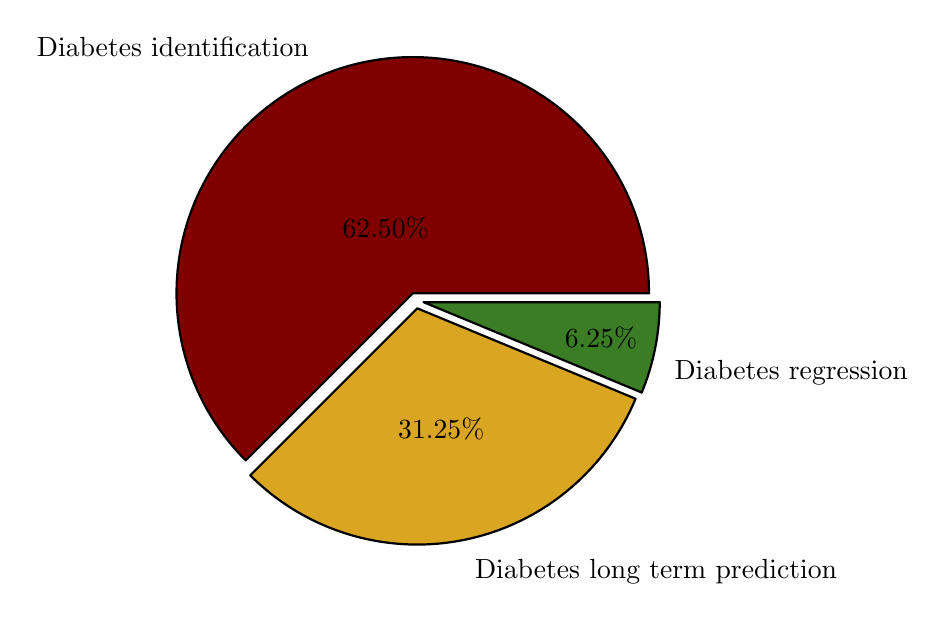
\begin{tikzpicture}
			\pie[explode=0.1, color ={Maroon!100,Goldenrod!100,OliveGreen!100}]{62.50/Diabetes identification,
					31.25/Diabetes long term prediction,
					6.25/Diabetes regression}
				\end{tikzpicture}}
				\caption{Percent of reviewed studies by purpose}
				\label{percent}
				
			    
		\end{figure}
		
			

		

%%%%%%%%%%%%%%%%%%%%%%%%%%%%%%%%%%%%%%%%%%
\section{Discussion}
\marginnote{Interpret the findings based on evidences(tables)}[0cm]
 The findings are oriented towards the following thematic axes.
 \begin{enumerate}
	\item Types of hypotheses addressing diabetes through Machine Learning using tabular data.
	\item Data preprocessing.
	\item Features involved.
	\item Selection and identification of most important Features.
    \item Methodology structure towards model building.
    \item Evaluation metrics. 
    \item Best models.
\end{enumerate}
In the end, relevant literature referring review studies are compared with ours. 
\subsection{Types of hypotheses addressing diabetes through Machine Learning using tabular data}
To start with,  recent applications on diabetes using tabular datacan be categorized to three discrete hypotheses. Current state 
diabetes identification, long term diabetes prediction and biomarkers regression. 
As Figure \ref{percent} depicts, the majority of hypotheses are in the context of current state diabetes identification with 
62.50\%, then long term diabetes prediction with 31.25\% and lastly diabetes biomarkers regression with 6.25\% in a sum of 16 articles. This
distribution is quite reasonable, because each hypothesis has different data collection requirements. First of all, the 
current state diabetes identification requires only present health condition, while in long term case, the class variable 
refering to diabetes state is filled many years after measurements completion, maintaining a baseline-follow up method. Thus,
the current state study has simpler data collection process than the long term one. Then, biomarkers regression such as 
FPG or HbA1c has even more complex dataset creation, because  the target variable should be measured continually and systematically
by the individuals with an invasive way. Moreover, the features values should be filled every time along with the measurements by 
indivudials, something that could lead to false or uncompleted data, due to lack of professional intervetion. Among them, the most
challening and interesting use case is the long term forecasting, because it would provide an early assessment of diabetes development.


\subsection{Data preprocessing}
Most research articles studied, give high importance in data preprocessing techniques such as empty values imputation, data balancing and
transformation, probing a variety of them.
The imputation is done with Mean/Mode or the more complex one MICE, while 
most of reviewed researches do not handle this issue, rather drop the empty values due to high data quantity. The evidences show 
that there is not a go-to method, but it depends on every specific problem setting, however MICE utilization in datasets with 
relatively low percent of missing data could simulate possible hidden patterns between features and therefore produce more realistic 
datasets.
\par Data balancing is undoubtly one of the most important stages, even thought the models have the highlights, because balancing
adjusts  the bias of the whole experiment. As from literature deducted, general approaches include oversampling minority instances,
undersampling majority instances, synthesizing artificial data (SMOTE) in order to product equal instances for all classes.
Interestingly, Fazakis et al. \cite{fazakis} successfully used undersampling technique to match real life positive diabetic cases age wise,
because with only 2,000 instances an equal size of classess could lead to significant bias towards positive diabetic cases. Also, 
Fazakis et al \cite{fazakis} and Lai et al \cite{Lai} utilized adjusted decision threshold of their classifier, yielding very good
results. 

\par Data transformation techniques included only in \cite{Dinh,Benita} (Standardization) and in \cite{Rufo,computation11050096}(MinMax).
Standardization contributes in general in all models, while MinMax normalization does not affect tree based models. This in 
contrary to \cite{Rufo,computation11050096}, which trained LightGBM and Random Forest, respectively, mainly for fair comparisons
against other MinMax dependent  models (SVM and KNN).


\subsection{Features involved}
Most datasets have a size of some thousands records (excluding \cite{Dritsas} with only 520) and include a variety of data representing
many aspects of humans. Datasets are mainly provided by clinics, hospitals and institutes such as NHANES \cite{Qin,Zou,DeSilva}.
The features involved are sociodemographic like age, sex, education level, salary and marital status, anthropometric/biometric like 
height, weight, BMI, waist circumference, systolic and diastolic pressure, and pulse rate, laboratory results like FPG, HbA1c, HDL,
LDL, total cholesterol, triglycerides, urea measurements, creatinine and gamma-GTP, lifestyle behaviour such as sleep time, smoking,
drinking and physical activity, family history of diabetes and dietary consumption data such as folate, carbohydrates and sugar
\cite{Qin,DeSilva}.
Most of those features are verified by medical literature that associate with diabetes (\cite{idf}), while others such as urea measurements,
gamma-GTP and dietary habits are under investigation. An advantage of tabular data is the low storage overhead comparing to images
which would demand thousands times more memory to be stored. However, such a plethora of features demands a systematic and time 
consuming registration effort, while also the participants could not be available to all measurements.

\subsection{Selection and identification of most important features}

Regarding the aforementioned problem, the application of feature selection techniques could contribute remove features which seem to be
unrelated to diabetes and thus help the data collection process, as well as the computational efficiency of model building.
As can be seen from Figure \ref{techRanking}, the top performed models utilized a variety of methods which belong to Wrapper,
Filter and Embedded. The most notable finding is that the majority of researchers chose to promote models trained on the whole 
feature set, rather than to a reduced version. A reason for that is the scope of each study. For example De Silva et al \cite{DeSilva}
examined dietary features contribution, while \cite{Dritsas} presented the influence of common diabetic symptoms.
However, the most useful result of such a study is the interpretability of associated factors, in order to moderate them towards
risk minimization. Luckily, with the new advancements of Machine Learning, the prediction models are not any more black boxes, but
with feature important methods, every feature contribution can be quantified. For instance, \cite{DeSilva} using odds ratio metric,
found folate consumption, self reported diet health and total fat consumption, while \cite{Dritsas} highlights the significance of
polyuria, polydipsia sudden weight loss and gender as best indicators of diabetes, using Pearson correlation,
Gain ratio, Random Forest and Naive Bayes AUC. Another finding, is the usual deployment of SHAP method,
(like in\cite{LAMA2021e07419,Qin,Shin,Mao}), which provides a common interface for all types of models to quantify feature influence, as
well as the influence of features on a particular participant \cite{LAMA2021e07419}. Summing up all of them, 
in Figure \ref{featureRanking} an enumeration of best predictor categories during this review can be seen.
Glycose related biomarkers FPG and HbA1c, as expected, found to be the most important predictors as they are known to be the principal
indicators of diabetes \cite{idf}. Age, BMI, heart operation metrics, Lipid profile and diabetes heredity seem to agree both on 
such data driven techniques as medical practice, in contrary to ethnicity which is not highlighted on the reviewed studies.
Finally, urinary parameters seem to be promising about their predictive capabilities (\cite{Dritsas,zhang}), while dietary factors should be more 
investigated \cite{DeSilva,zhang,LAMA2021e07419}. 

\begin{figure}[H]
	\begin{subfigure}[b]{.35\textwidth}
		\resizebox{\textwidth}{!}{
		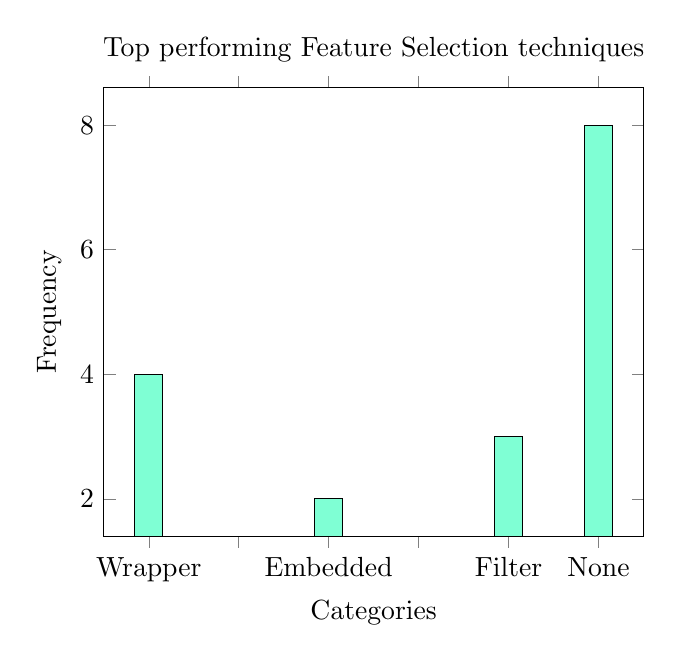
\begin{tikzpicture}
			\begin{axis}[xlabel={Categories},ylabel={Frequency},ybar, title={Top performing Feature Selection techniques}, symbolic x coords={Wrapper,,Embedded,,Filter,None}] 
				\addplot[fill=Aquamarine!100] coordinates{(Wrapper,4) (Filter,3) (Embedded,2) (None, 8)};
			\end{axis}
		\end{tikzpicture}}
		\caption{}
		\label{techRanking}
	\end{subfigure}
	\begin{subfigure}[b]{.65\textwidth}
		\resizebox{\textwidth}{!}{
		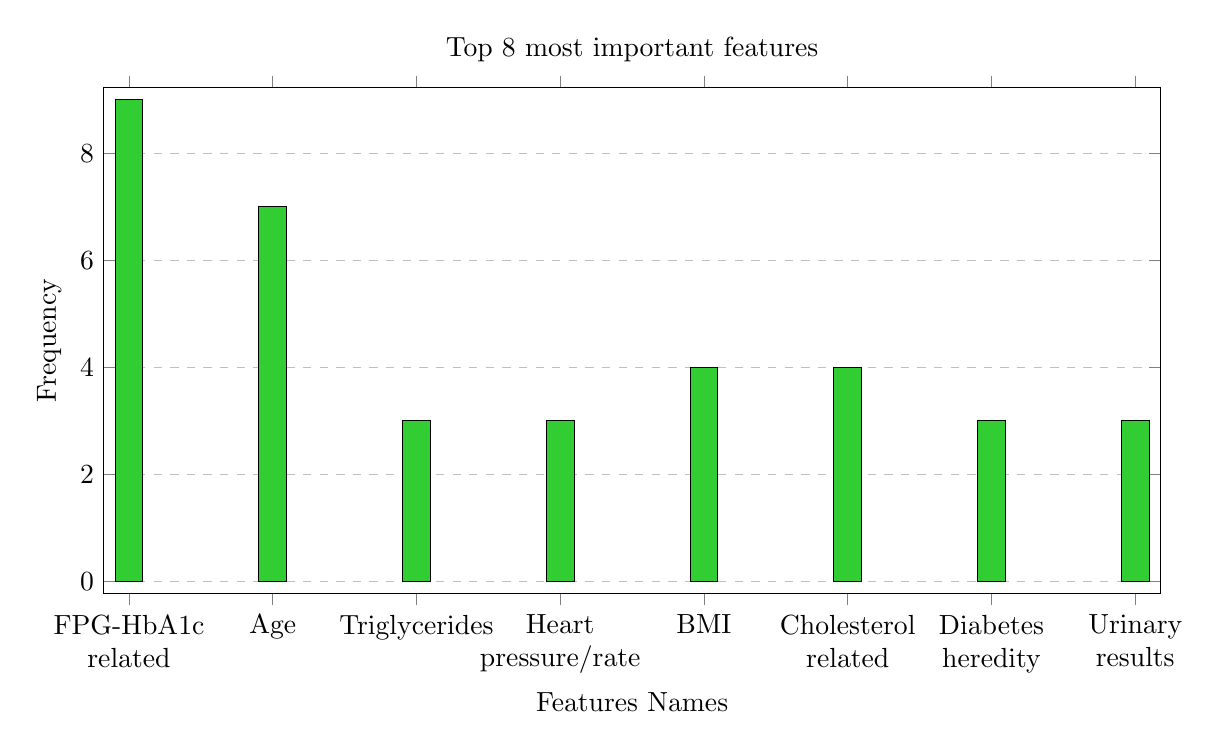
\begin{tikzpicture}
			\begin{axis}[
				ybar,
				title={Top 8 most important features},
				ymin=0,
				ymax=9,
				width=15cm,
				height=8cm,
				xlabel={Features Names},
				xticklabel style={align=center},
				ylabel={Frequency},
				xtick=data,
				xticklabels={FPG-HbA1c\\ related, Age, Triglycerides,Heart\\ pressure/rate, BMI, Cholesterol\\ related, Diabetes\\ heredity, Urinary\\ results},
				enlargelimits=0.025,
				legend style={at={(0.5,-0.15)},
				  anchor=north,legend columns=-1},
				ymajorgrids=true,
				grid style=dashed,
			]
			\addplot+[
				fill=LimeGreen!100,
				draw=black,
			] coordinates {
				(1, 9)
				(2, 7)
				(3, 3)
				(4, 3)
				(5, 4)
				(6, 4)
				(7, 3)
				(8, 3)

			};
			\end{axis}
			\end{tikzpicture}}
			\caption{}
			\label{featureRanking}
	\end{subfigure}
	\caption{}
\end{figure}

\subsection{Methodology structure towards model building}

In general this stage offers wide freedom of management. However, our findings present with clarity a common pattern that exists 
in model building. Firstly, a number of researches use many different feature subsets, that arose either from a variety of 
feature selection methods or from medical bibliography or from the hypothesis, which is examined \cite{Zou,Dinh,zhang,computation11050096,
kopitar2020early,fazakis}. Datasets with laboratory data are compared against non invasive data, to evaluate if the latter can provide 
relatively reliable results \cite{Dinh}. According to table \ref{tab1}, the vast majority studies prefer train/test split usually with 
80/20 ratio, hyperparameter tuning using mostly grid search and 10-fold cross validation. Due to the data quantity, the split
percent as well as the number of folds are considered as good choice. The figure \ref{workflow} presents a typical workflow towards
model building, as extracted by the reviewed literature, (e.g balancing at preprocessing, wrapper or none feature selection technique,
the training procedure, the evaluation metrics and the popular feature importance methods).

\begin{figure}[H]
	\centering
		\resizebox{.85\textwidth}{!}{
		\begin{tikzpicture}[node distance=2cm]
			\node (preprocessing)[align=center,rectangle, rounded corners,minimum width=1cm,minimum height=1cm,text centered,draw=black,fill=blue!30]{
				\textbf{Data preprocessing}\\
				\vspace{.5cm}
				\\
				\begin{tikzpicture}
					\node (nested)[align=center,rectangle, rounded corners,minimum width=1cm,minimum height=1cm,text centered,draw=black,fill=blue!40]{
						\footnotesize	Balancing
					};
				\end{tikzpicture}
			};
			\node (feature selection)[xshift=2cm,align=center,rectangle, rounded corners,minimum width=1cm,minimum height=1cm,text centered,draw=black,fill=Peach!30, right of=preprocessing]{
				\textbf{Feature Selection}\\
				\vspace{.5cm}
				\\
				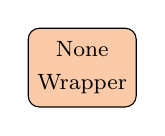
\begin{tikzpicture}
					\node (nested2)[align=center,rectangle, rounded corners,minimum width=1cm,minimum height=1cm,text centered,draw=black,fill=Peach!40]{
						\footnotesize    None\\
						\footnotesize	Wrapper 
					};
				\end{tikzpicture}
			};
			\node (training)[xshift=4cm,align=center,rectangle, rounded corners,minimum width=1cm,minimum height=1cm,text centered,draw=black,fill=JungleGreen!30, right of=feature selection]{
				\textbf{Training methods}\\
				\vspace{.5cm}
				\\
				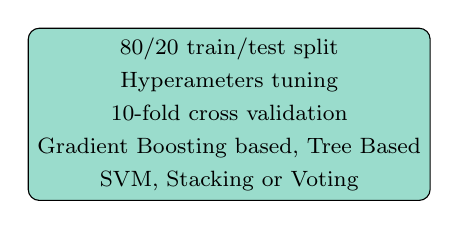
\begin{tikzpicture}
					\node (nested3)[align=center,rectangle, rounded corners,minimum width=1cm,minimum height=1cm,text centered,draw=black,fill=JungleGreen!40]{
						\footnotesize 80/20 train/test split\\
						\footnotesize Hyperameters tuning\\
						\footnotesize 10-fold cross validation\\
						\footnotesize Gradient Boosting based, Tree Based\\
						\footnotesize SVM, Stacking or Voting
					};
				\end{tikzpicture}};
				\node (evaluation)[yshift=-2cm,align=center,rectangle, rounded corners,minimum width=1cm,minimum height=1cm,text centered,draw=black,fill=Goldenrod!30, below of=training]{
					\textbf{Evaluation metrics}\\
					\vspace{.5cm}
					\\
					
					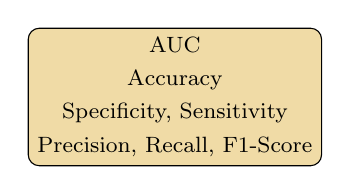
\begin{tikzpicture}
						\node (nested4)[align=center,rectangle, rounded corners,minimum width=1cm,minimum height=1cm,text centered,draw=black,fill=Goldenrod!40]{
							\footnotesize AUC\\
							\footnotesize Accuracy\\
							\footnotesize Specificity, Sensitivity\\
							\footnotesize Precision, Recall, F1-Score
						};
					\end{tikzpicture}};
					\node (importance)[yshift=-2cm,align=center,rectangle, rounded corners,minimum width=1cm,minimum height=1cm,text centered,draw=black,fill=ForestGreen!30, below of=feature selection]{
						\textbf{Feature Importance}\\
						\vspace{.5cm}
						\\
						
						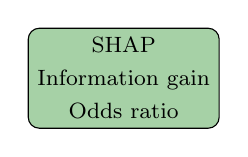
\begin{tikzpicture}
							\node (nested5)[align=center,rectangle, rounded corners,minimum width=1cm,minimum height=1cm,text centered,draw=black,fill=ForestGreen!40]{
								\footnotesize SHAP\\
								\footnotesize Information gain\\
								\footnotesize Odds ratio
							};
						\end{tikzpicture}};
	
			\draw[->] (preprocessing)--(feature selection);
			\draw[->] (feature selection)--(training)  node[align=center,left, yshift=1cm, xshift = -2.6cm]{Try\\ different\\ feature\\ sets};;
			\draw[->] (feature selection)--(importance) node[left, yshift=2cm, xshift = -.5cm]{Along with}; 
			\draw[->] (training)--(evaluation);
			\draw[->] (evaluation)--(importance);
			\node (results)[yshift=-2cm,align=center,circle,minimum width=1cm,minimum height=1cm,text centered,draw=black,fill=Goldenrod!30, below of =preprocessing]{\textbf{Results}\\\vspace{.2cm}\\\footnotesize Best model\\
			\footnotesize Best feature set\\
			\footnotesize Feature interpretation};
			%\node ()
		\end{tikzpicture}}
		\caption{Typical methodology workflow}
		\label{workflow}
	\end{figure}
\vfil

\subsection{Evaluation metrics}

In most of examined studies, the evaluation metrics are the typical ones such as AUC, Accuracy, Sensitivity or Recall, Specificity,
Precision and F1-Score. These provide a complete understanding of performance. However, in such use cases as disease detection,
Sensitivity must have the priority because the higher it is, the less possible is for an individual with diabetes to diagnosed
as healthy. Other metrics used are misclassification rate in \cite{Lai},  AIC in \cite{Qin}, robustness in
\cite{LAMA2021e07419} and Youden index in \cite{fazakis}. Generally, researchers should be urged  to include different existing or new, 
custom metrics.

\subsection{Best models}

Figure \ref{bar:top_models} depicts the general categories
of top models as elected on reviewed studies, clustered by the hypothesis. For the identification purpose, Gradient Boosting 
models have a clear advantage, with Random Forest coming second. For long term forecasting, Stacking and Voting share the top
with Random Forest, while for biomarkers regression the one and only model preferred belongs to Gradient Boosting family. SVM, kNN
as well as logistic regression are not yet preferred, first of all due to their worse performance and secondly because these 
models demand data transformation such as MinMax normalization due to data heterogenity, which would be time and resource 
consuming in datasets of some decades of thousands. On the other hand Gradient Boosting and tree like models stay 
unaffected by the different numerical ranges of features.

\begin{figure}[!h]
	\centering
	\resizebox{.5\textwidth}{!}{
				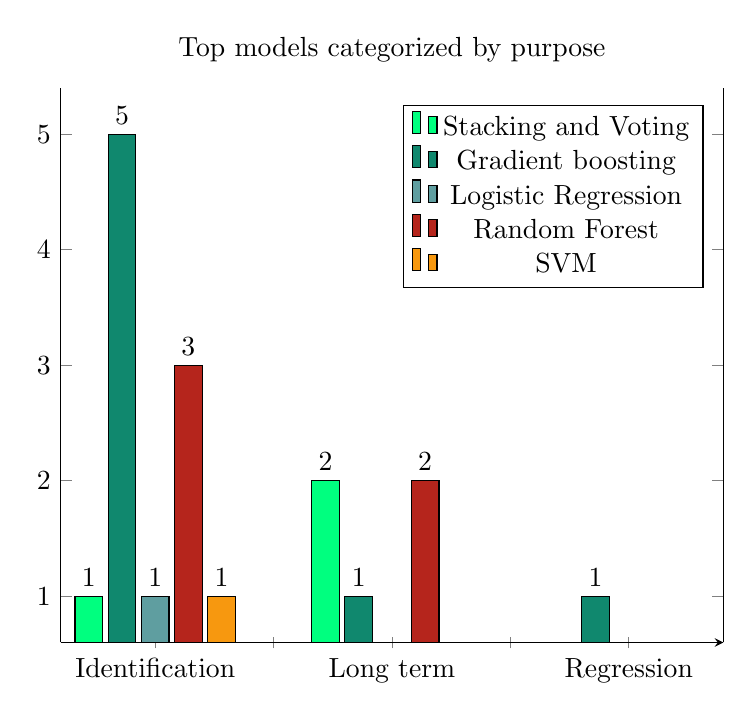
\begin{tikzpicture}
					\begin{axis}[ybar, title={Top models categorized by purpose}, symbolic x coords={{},Identification,,Long term,,Regression,,},
						legend pos = north east,ytick={0,1,2,3,4,5}, axis x line=bottom, nodes near coords, enlarge x limits=0.2,width=10cm, ] 
					  \addplot[fill=SpringGreen!100] coordinates {(Identification,1)  (Long term,2)  (Regression,)}; %ensemble
					  \addplot[fill=PineGreen!100] coordinates {(Identification, 5) (Long term, 1) (Regression,1)}; %gradient boosting
					  \addplot[fill=CadetBlue!100] coordinates {(Identification, 1) (Long term,) (Regression,)}; %Logistic
					  \addplot[fill=BrickRed!100] coordinates {(Identification, 3) (Long term, 2) (Regression,)}; %RF
					  \addplot[fill=YellowOrange!100] coordinates {(Identification, 1) (Long term,) (Regression,)}; %SVM
					  \legend{Stacking and Voting, Gradient boosting, Logistic Regression, Random Forest, SVM}; \end{axis} 
					\end{tikzpicture}}
				    \caption{Top performing models categorized by purpose}
					\label{bar:top_models}
\end{figure}

\subsection{Comparing to previous reviews}

Both reviews \cite{Fregoso,KAVAKIOTIS2017104} examine a broader context of Artificial Intelligence and T2D mellitus, including 
deep learning, unsupervised learning and association rules. Kavakiotis et al \cite{KAVAKIOTIS2017104}, although it is older publication,
deals with a more general overview of applied methods, which includes hypotheses about diabetic complications prediction, data driven
investigation of both drugs and therapies, genetic background and enviroment, and health care management. In contrast to our research,
they found SVM to be the best model towards diabetes hypotheses. Fregoso et al \cite{Fregoso} as a publication of 2021, agrees with us
in the finding that tree based, ensemble models have the top performance. In contrary to us, they found Linear Regression coefficients
and PCA as the most popular feature selection techniques and heterogenity in model assessment metrics. SHAPley values are not of 
great concern in both studies, while as proved to our study, it is a wide acceptable interpretation method. Our limitations,
include the examination of quite new articles along  with few high quality older ones, that use tabular data and machine learning models.
An advancement of our research is that it is trying to provide an in-depth, detailed methodology description of all overviewed articles, 
unveil common successfull patterns, highlight new asceding features and subsequently provide new research areas.






%%%%%%%%%%%%%%%%%%%%%%%%%%%%%%%%%%%%%%%%%%
\section{Conclusions}
By their nature, the identification, or even better a very early forecast of T2D mellitus, are very interesting cases of study, 
because people could be able to stay informed about their health situation and try to prevent further negative development.
In this study we overviewed the recent Machine Learning applications towards T2D mellitus prediction using tabular data such as 
demographic, biometric, laboratory, lifestyle and dietary data, with a goal to investigate common patterns towards ML models 
implementation and discover both asceding methods and features. Interestingly we found Gradient Boosting and Tree based
models as the most successfull ones, which are trained and optimized usually with grid search, as well as that SHAPley and Wrapper
algorithms are the quite popular feature interpretation and evaluation methods. Apart from classical laboratory biomarkers,
urinary results and non-invasive dietary informations are promising features opening new research areas, which possibly could lead 
to prevention or easier management of T2D mellitus. 

%%%%%%%%%%%%%%%%%%%%%%%%%%%%%%%%%%%%%%%%%%
%\section{Future Directions}

%This section is not mandatory, but may be added if there are patents resulting from the work reported in this manuscript.



%%%%%%%%%%%%%%%%%%%%%%%%%%%%%%%%%%%%%%%%%%
\vspace{6pt} 

%%%%%%%%%%%%%%%%%%%%%%%%%%%%%%%%%%%%%%%%%%
%% optional
%\supplementary{The following supporting information can be downloaded at:  \linksupplementary{s1}, Figure S1: title; Table S1: title; Video S1: title.}

% Only for the journal Methods and Protocols:
% If you wish to submit a video article, please do so with any other supplementary material.
% \supplementary{The following supporting information can be downloaded at: \linksupplementary{s1}, Figure S1: title; Table S1: title; Video S1: title. A supporting video article is available at doi: link.}

%%%%%%%%%%%%%%%%%%%%%%%%%%%%%%%%%%%%%%%%%%
\authorcontributions{For research articles with several authors, a short paragraph specifying their individual contributions must be provided. The following statements should be used ``Conceptualization, X.X. and Y.Y.; methodology, X.X.; software, X.X.; validation, X.X., Y.Y. and Z.Z.; formal analysis, X.X.; investigation, X.X.; resources, X.X.; data curation, X.X.; writing---original draft preparation, X.X.; writing---review and editing, X.X.; visualization, X.X.; supervision, X.X.; project administration, X.X.; funding acquisition, Y.Y. All authors have read and agreed to the published version of the manuscript.'', please turn to the  \href{http://img.mdpi.org/data/contributor-role-instruction.pdf}{CRediT taxonomy} for the term explanation. Authorship must be limited to those who have contributed substantially to the work~reported.}

\funding{Please add: ``This research received no external funding'' or ``This research was funded by NAME OF FUNDER grant number XXX.'' and  and ``The APC was funded by XXX''. Check carefully that the details given are accurate and use the standard spelling of funding agency names at \url{https://search.crossref.org/funding}, any errors may affect your future funding.}

\institutionalreview{In this section, you should add the Institutional Review Board Statement and approval number, if relevant to your study. You might choose to exclude this statement if the study did not require ethical approval. Please note that the Editorial Office might ask you for further information. Please add “The study was conducted in accordance with the Declaration of Helsinki, and approved by the Institutional Review Board (or Ethics Committee) of NAME OF INSTITUTE (protocol code XXX and date of approval).” for studies involving humans. OR “The animal study protocol was approved by the Institutional Review Board (or Ethics Committee) of NAME OF INSTITUTE (protocol code XXX and date of approval).” for studies involving animals. OR “Ethical review and approval were waived for this study due to REASON (please provide a detailed justification).” OR “Not applicable” for studies not involving humans or animals.}

\informedconsent{Any research article describing a study involving humans should contain this statement. Please add ``Informed consent was obtained from all subjects involved in the study.'' OR ``Patient consent was waived due to REASON (please provide a detailed justification).'' OR ``Not applicable'' for studies not involving humans. You might also choose to exclude this statement if the study did not involve humans.

Written informed consent for publication must be obtained from participating patients who can be identified (including by the patients themselves). Please state ``Written informed consent has been obtained from the patient(s) to publish this paper'' if applicable.}

\dataavailability{In this section, please provide details regarding where data supporting reported results can be found, including links to publicly archived datasets analyzed or generated during the study. Please refer to suggested Data Availability Statements in section ``MDPI Research Data Policies'' at \url{https://www.mdpi.com/ethics}. If the study did not report any data, you might add ``Not applicable'' here.} 

\acknowledgments{In this section you can acknowledge any support given which is not covered by the author contribution or funding sections. This may include administrative and technical support, or donations in kind (e.g., materials used for experiments).}

\conflictsofinterest{Declare conflicts of interest or state ``The authors declare no conflict of interest.'' Authors must identify and declare any personal circumstances or interest that may be perceived as inappropriately influencing the representation or interpretation of reported research results. Any role of the funders in the design of the study; in the collection, analyses or interpretation of data; in the writing of the manuscript; or in the decision to publish the results must be declared in this section. If there is no role, please state ``The funders had no role in the design of the study; in the collection, analyses, or interpretation of data; in the writing of the manuscript; or in the decision to publish the~results''.} 

%%%%%%%%%%%%%%%%%%%%%%%%%%%%%%%%%%%%%%%%%%
%% Optional
\sampleavailability{Samples of the compounds ... are available from the authors.}

%% Only for journal Encyclopedia
%\entrylink{The Link to this entry published on the encyclopedia platform.}

\abbreviations{Abbreviations}{
The following abbreviations are used in this manuscript:\\

\noindent 
\begin{tabular}{@{}ll}
MDPI & Multidisciplinary Digital Publishing Institute\\
DOAJ & Directory of open access journals\\
TLA & Three letter acronym\\
LD & Linear dichroism
\end{tabular}
}

%%%%%%%%%%%%%%%%%%%%%%%%%%%%%%%%%%%%%%%%%%
%% Optional
%\appendixtitles{no} % Leave argument "no" if all appendix headings stay EMPTY (then no dot is printed after "Appendix A"). If the appendix sections contain a heading then change the argument to "yes".
%\appendixstart
%\appendix
%\section[\appendixname~\thesection]{}
%\subsection[\appendixname~\thesubsection]{}
%The appendix is an optional section that can contain details and data supplemental to the main text---for example, explanations of experimental details that would disrupt the flow of the main text but nonetheless remain crucial to understanding and reproducing the research shown; figures of replicates for experiments of which representative data are shown in the main text can be added here if brief, or as Supplementary Data. Mathematical proofs of results not central to the paper can be added as an appendix.



%\section[\appendixname~\thesection]{}
%All appendix sections must be cited in the main text. In the appendices, Figures, Tables, etc. should be labeled, starting with ``A''---e.g., Figure A1, Figure A2, etc.

%%%%%%%%%%%%%%%%%%%%%%%%%%%%%%%%%%%%%%%%%%
\begin{adjustwidth}{-\extralength}{0cm}
%\printendnotes[custom] % Un-comment to print a list of endnotes

\reftitle{References}

% Please provide either the correct journal abbreviation (e.g. according to the “List of Title Word Abbreviations” http://www.issn.org/services/online-services/access-to-the-ltwa/) or the full name of the journal.
% Citations and References in Supplementary files are permitted provided that they also appear in the reference list here. 

%=====================================
% References, variant A: external bibliography
%=====================================
\bibliography{references.bib}

%=====================================
% References, variant B: internal bibliography
%=====================================

% If authors have biography, please use the format below
%\section*{Short Biography of Authors}
%\bio
%{\raisebox{-0.35cm}{\includegraphics[width=3.5cm,height=5.3cm,clip,keepaspectratio]{Definitions/author1.pdf}}}
%{\textbf{Firstname Lastname} Biography of first author}
%
%\bio
%{\raisebox{-0.35cm}{\includegraphics[width=3.5cm,height=5.3cm,clip,keepaspectratio]{Definitions/author2.jpg}}}
%{\textbf{Firstname Lastname} Biography of second author}

% For the MDPI journals use author-date citation, please follow the formatting guidelines on http://www.mdpi.com/authors/references
% To cite two works by the same author: \citeauthor{ref-journal-1a} (\citeyear{ref-journal-1a}, \citeyear{ref-journal-1b}). This produces: Whittaker (1967, 1975)
% To cite two works by the same author with specific pages: \citeauthor{ref-journal-3a} (\citeyear{ref-journal-3a}, p. 328; \citeyear{ref-journal-3b}, p.475). This produces: Wong (1999, p. 328; 2000, p. 475)

%%%%%%%%%%%%%%%%%%%%%%%%%%%%%%%%%%%%%%%%%%
%% for journal Sci
%\reviewreports{\\
%Reviewer 1 comments and authors’ response\\
%Reviewer 2 comments and authors’ response\\
%Reviewer 3 comments and authors’ response
%}
%%%%%%%%%%%%%%%%%%%%%%%%%%%%%%%%%%%%%%%%%%
\end{adjustwidth}
\end{document}

